We start by briefly introducing reasoning techniques (\textit{e.g.}, chain-of-thought \citep{DBLP:conf/nips/Wei0SBIXCLZ22}, ReAct \citep{DBLP:conf/iclr/YaoZYDSN023}, \textit{etc}).
%good reasoning rationales can improve the ability of autoregressive-based LLMs to produce correct responses to complex tasks.
Given a user query $\px$, the standard procedure to sample the response $\py$ is to leverage an autoregressive pretrained LLMs $\pi_\theta$ (parameterized by $\theta$): $\py \sim \pi_\theta (\cdot ~|~ \px)$.
As for prompt-based reasoning techniques such as chain-of-thought \citep{DBLP:conf/nips/Wei0SBIXCLZ22},
the LLM $\pi_\theta$ is firstly asked to generate thoughts (\textit{a.k.a} reasoning rationale) before generating the answers to the response:
\begin{align*}
    \px^\prime := \texttt{Reason}(\px) &= \px \oplus \texttt{Prompt}~\texttt{Template}~\texttt{of}~\texttt{Thought},\\
    ~~~ \pz \sim \pi_\theta &(\cdot ~| ~\px^\prime) ,~~~~\py \sim \pi_\theta (\cdot ~| ~\px^\prime \oplus \pz)\,,
\end{align*}
where $\pz$ is the thought or the reasoning rationale path, $\oplus$ indicates the concatenate operator, and the prompt template of the thought can be some hint prompt such as ``\texttt{Let's think s
tep by step}'' \footnote{We omit the difference between $x^\prime$ and $x$ for convenience in the latter notation.}.Empirically, people observe that there is a higher chance for the LLM $\pi_\theta$ to generate the desired answer $\py$ following the above procedure than directly sampling the response $\py \sim \pi_\theta(\cdot ~| ~\px)$.  
From a statistical perspective, we hypothesize that good reasoning rationales can significantly improve the probability of generating good answers $\py$: $~\exists~ \pz, ~~\textit{s.t.}~ \pi_\theta(\py |~\px \oplus \pz) \gg \pi_\theta (\py | ~\px)$.
\begin{wrapfigure}{r}{0.40\textwidth}
    \centering
    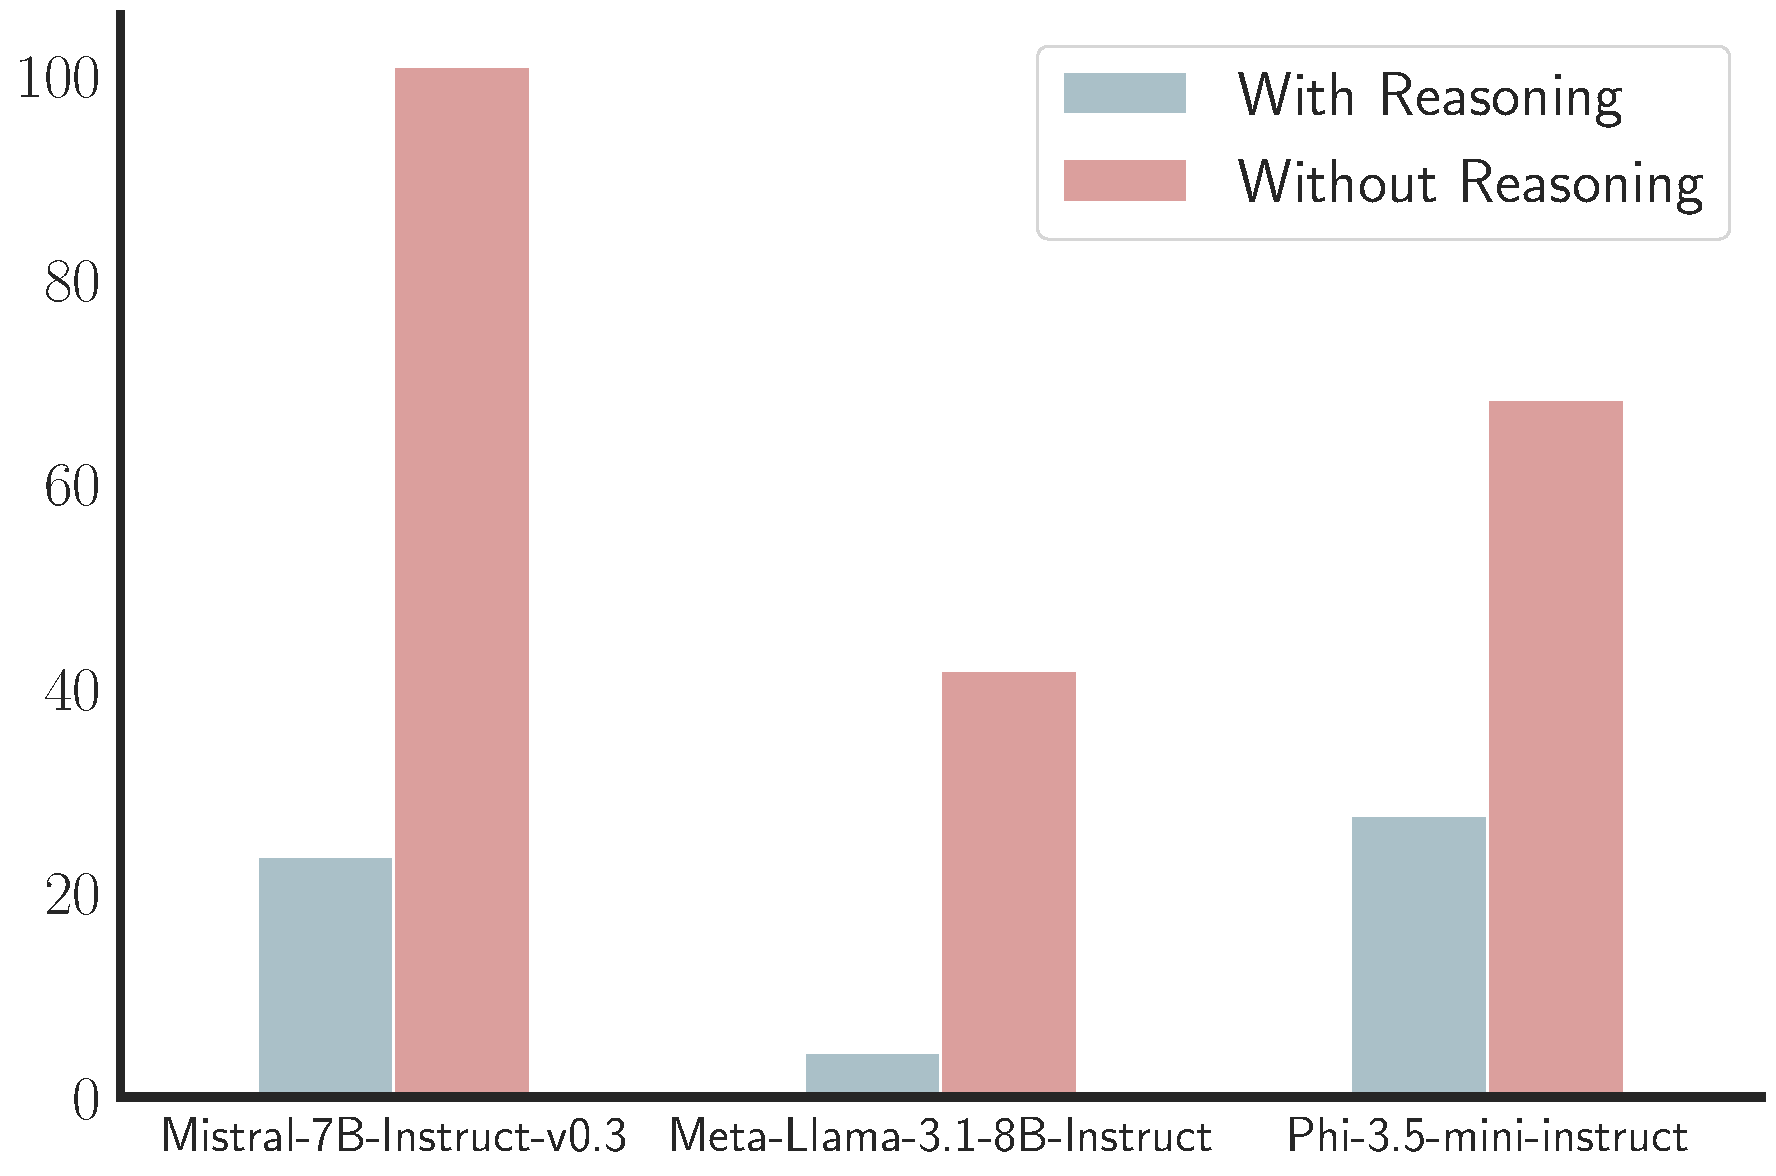
\includegraphics[width=\linewidth]{figures/logprob_diff.pdf}
    \vspace{-1em}
    \caption{\footnotesize{Average negative log probabilities of  LLMs to generate correct responses.}}
    %The red bar indicates the mean negative log probability that a model correctly answers after only the question, whereas the gray bar indicates the mean negative log probability after the model sees both the question and the golden rationale (lower values imply higher likelihood to answer correctly). \yy{@haolin, add more explanations here, and what's y axis.} consider make this a minipage or a wrap figure}
    \label{fig:logprob_comparison}
    \vspace{-3em}
\end{wrapfigure}

To validate the hypothesis, we check the probability of the correct answers $\py$ on pretrained LLMs with or without reasoning rationales.
In \Cref{fig:logprob_comparison},
we visualize the negative log probability of the correct answers on three different LLMs on GSM8K dataset \citep{cobbe2021training}.
We have observed that when the LLMs are conditioned on the reasoning rationales, the probability of the correct answer is remarkably larger than without reasoning rationales.
This suggests that good reasoning rationales help the LLMs generate desired answers for complex tasks by increasing their probability, giving them a higher chance of generating the correct answers. 

\iffalse
The first question we would like to address is: Does LLM possess hidden reasoning capabilities or understand the semantics of reasoning?

We observe that, given a query-rationale-response triplet $(x,z,y)$, an autoregressive LLM is much more likely to produce the correct response $y$ when conditioned on both query $x$ and rationale $z$ than when conditioned on the query alone.

\fi 

%According to \Cref{fig:logprob_comparison}, the probability of generating correct responses in GSM8K increases markedly in three distinct LLMs when a golden reasoning trajectory is provided. This suggests that the log probability LLMs assign to correct answers when conditioned on the input could act as a natural reward function. This finding motivates us to develop a framework that optimizes the rationale $z$ using self-rewarding. We start by formulating prompt-based reasoning methods as a latent variable model.

%\subsection{Prompt-based reasoning as a latent variable model}
%\label{sec:formulation}
\iffalse
Given the user query, a prompt-based LLM reasoning algorithm is a function $\reason$ that maps the user query to the actual input $x$ model receives using a prompt template, such that $x$ induces an intermediate rationale $z$ and an intermediate distribution $\llm(\cdot | x\oplus z)$ to generate the answer:
\[y \sim \llm(\cdot|x\oplus z),\]
where $z\sim\llm(\cdot|x)$. For example, in CoT or ReAct \citep{DBLP:conf/iclr/YaoZYDSN023}, the LLM is asked to provide thoughts before generating the answer or action:
\[x=\reason(\texttt{query}) = \texttt{query}\oplus \text{prompt template for thoughts}.\]
We hope, and empirical evidence shown in \Cref{fig:logprob_comparison} suggests that by routing to first generate rationale $z$, at the end $\llm$ generates the desired answer $y$ with higher probabilities:
$
\exists z, \text{such that }\llm(y|x\oplus z) \geq \llm(y|x).
$
The reasoning process can be seen as sampling the rationale $z$ from a latent distribution $\llm(\cdot|x)$. With this reasoning process, we assume that: 
\begin{assumption}\label{ass:ll}
    The latent reasoning process will increase the probability of generating the groundtruth response $y^*$, that is
    \begin{equation}
        \label{eqn:assumption}
        \E_{z\sim\llm(\cdot|x)}\llm(y^*|x\oplus z) \gg \llm(y^*|x).    
    \end{equation}
\end{assumption}
\fi 


% \begin{remark}
%     When $\reason$ is CoT, the expectation in \Cref{eqn:assumption} is the limiting distribution of CoT-SC \citep{DBLP:conf/iclr/0002WSLCNCZ23}. \haolincomment{write a short proof here when time allows}
% \end{remark}
%Notice that we have the following relationship between the left hand side of \cref{eqn:assumption} and 

%We may wonder whether it is doable to further improve the reasoning ability of the LLMs by leveraging the above observation. 
%We may want to improve the reasoning ability of existing LLMs further, based on the observations. 
The above observation inspires us that we can potentially further improve the reasoning ability of existing LLMs. 
One may find some surrogate objective to enhance the quality of the reasoning rationales or improve the ability of LLMs to leverage good reasoning rationales. 
In the following \Cref{prop:cot-sc},
we show that \textit{Self-Consistency} Chain-of-Thought (CoT-SC) \citep{DBLP:conf/iclr/0002WSLCNCZ23}, which takes a majority vote of multiple reasoning rationales to improve the reasoning ability,
approximates some surrogate objective.
%the popular inference-time methods CoT-SC \citep{DBLP:conf/iclr/0002WSLCNCZ23} or major voting.

%\yy{todo: 1) add explanation of cot-sc; 2) add motivation of moving testing / inference to training. }

%Besides simple COT \citep{DBLP:conf/nips/Wei0SBIXCLZ22} which directly leverage, 
\begin{proposition}\label{prop:cot-sc}
    Denote the user query, model response, and reasoning rationale by $\px, \py,\pz$, respectively. 
    The distribution of the majority vote answer of the $K$ reasoning rationales obtained by CoT-SC approximates $p_{M}(\py | \px):= \E_{\pz\sim\llm(\cdot|~\px)}[\llm(\py|~\px\oplus \pz)]$, as $K \rightarrow \infty$.
    %When we use CoT to obtain reasoning rationales, 
    %the distribution of the 
    %When $\reason$ is CoT, $\E_{z\sim\llm(\cdot|x)}\llm(\cdot|x\oplus z)$ is the limiting distribution of CoT-SC as the number of sampled trajectories $K\rightarrow\infty$.
\end{proposition}
\begin{proof}
    Given a user query $\px$, CoT-SC essentially follows the procedure: 1) Sample $K$ \textit{i.i.d} reasoning rationales together with model responses:
    $(\pz_k, \py_k) \sim \pi_\theta (\cdot | \px),~1 \leq k \leq K$.
    2) Take the majority vote of $(\py_1,\ldots, \py_K)$.
    For a specific response $\py$, its frequency can be calculated as $F(\py):= \frac{1}{K}\sum^K_{k=1} \mathbbm{1} \{\py_k = \py\} $, where $\mathbbm{1}$ is the indicator function. Then the expectation of $F(\py)$ is 
   % Self-consistency essentially does the following: 1. Sample $K$ i.i.d. trajectories of (rationale, response): $(z_1,y_1),\ldots, (z_K, y_K)$ from $\llm(\cdot|x)$; 2. Take the majority vote of $y_i$s. Then for a specific response $y$, we have its frequency $F(y):= \frac{1}{K}\sum^K_{i=1} \mathbbm{1} \{y_i = y\} $, where $\mathbbm{1}$ is the indicator function. Then, the expectation of this frequency becomes
    \begin{equation*}
        \begin{split}
            \E_{\py_1,\ldots,\py_K} F(\py) &= \frac{1}{K}\sum^K_{k=1} \E_{\py_i} \mathbbm{1} \{\py_i = y\} = \frac{1}{K}\sum^K_{i=1} \prob_{\py_i\sim \llm(\cdot |\px\oplus \pz_i)}[\py_i = \py] \\
            &= \frac{1}{K}\sum^K_{i=1} \llm(\py| \px\oplus \pz_i) \overset{K\rightarrow\infty}{\longrightarrow} \E_{\pz\sim \llm(\cdot|\px)}\llm(\py|\px\oplus \pz).
        \end{split}
    \end{equation*}
\end{proof}
CoT-SC essentially leverages $p_{M}(\py | \px):= \int\llm(\pz|\px)\llm(\cdot|~\px\oplus \pz)d\pz$  
to obtain reasoning rationales and produce final correct answers.
Inspired by the conclusion, 
we could leverage surrogate objectives like $\E_{\pz\sim\llm(\cdot|~\px)}[\phi(\llm(\py|~\px\oplus \pz))]$ to further enhance the reasoning ability of LLMs, where $\phi$ is some monotonic transform such as logarithm ($\log(\cdot)$).
Further, we could also optimize the parameters of LLMs to enhance the reasoning abilities of existing LLMs during the training, so we can obtain LLMs with better reasoning abilities with the same inference time budget. 
In the following sections, we introduce the idea of optimizing LLMs to improve reasoning abilities without external feedback, by proposing a principled framework containing the surrogate objective.
